\documentclass[twocolumn]{article}
\usepackage{graphicx}
\begin{document}
\title{The Error Function}
\author{Wikipedia, the free encyclopedia}
\date{}
\maketitle
\begin{abstract}
All credits goes to the good people editing Wikipedia.
\end{abstract}

\section{If you remember this formula, then life will be good}
The first formula from the german wikipage:
\begin{equation}
\textrm{erf}(x) = \frac 2{\sqrt\pi} \int_0^x e^{-\tau^2}
\label{eq-error}
\end{equation}
Celebrate!

\section{The name 'error function'}
\textbf{The following is all taken from the English Wikipedia on the error function:}\\

The error function is used in measurement theory (using probability and statistics), and its use in other branches of mathematics is typically unrelated to the characterization of measurement errors.

In statistics, it is common to have a variable $Y$ and its unbiased estimator $\hat{Y}$. The error is then defined as $\varepsilon = \hat{Y} - Y$. This makes the error a normally distributed random variable with mean 0 (because the estimator is unbiased) and some variance $\sigma^2$; this is written as $\varepsilon \sim \mathcal{N}(0,\,\sigma^2)$. For the case where $\sigma^2 = \frac{1}{2}$, i.e. an unbiased error variable $\varepsilon \sim \mathcal{N}(0,\,\frac{1}{2})$, erf($x$) describes the probability of the error $\epsilon$ falling in the range [−$x$, $x$]; in other words, the probability that the absolute error is no greater than $x$. This is true for any random variable with distribution $\mathcal{N}(0,\,\frac{1}{2})$; but the application to error variables is how the error function got its name.

The previous paragraph can be generalized to any variance: given a variable (such as an unbiased error variable) $\varepsilon \sim \mathcal{N}(0,\,\sigma^2)$, evaluating the error function at erf$\left( \frac{x}{\sigma} \cdot \frac{1}{\sqrt{2}} \right)$ describes the probability of $\epsilon$ falling in the range [-$x$, $x$]. This is used in statistics to predict behavior of any sample with respect to the population mean. This usage is similar to the [[Q-function]], which in fact can be written in terms of the error function.

\section{How to cite figures and equations}
Hello world, this is a reference to figure \ref{fig-error}. Another reference to the first equation \ref{eq-error}.

\begin{figure}[h]
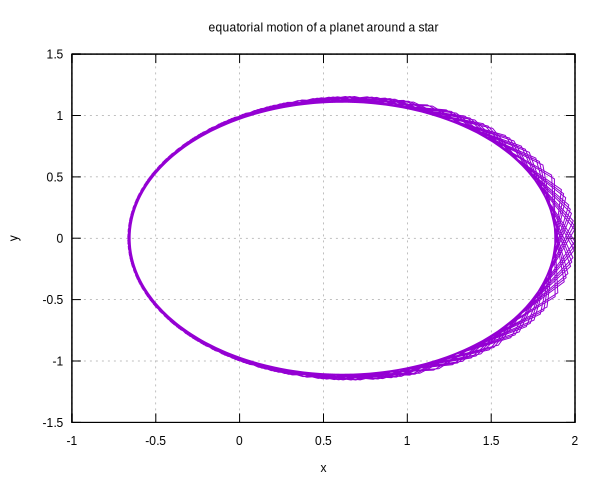
\includegraphics{plot.pdf}
\caption{The error function}
\label{fig-error}
\end{figure}

\end{document}